\documentclass[8pt]{article}
\usepackage[a4paper,landscape,margin=1in]{geometry}
\usepackage{cmbright}

\usepackage{amsmath}
\usepackage{nicefrac}
\usepackage{siunitx}

\usepackage{array}
\usepackage{booktabs}
\usepackage{longtable}

\usepackage{xcolor}
\definecolor{urlblue}{HTML}{0000ee}
\usepackage{hyperref}
\hypersetup{%
colorlinks = true,%
urlcolor   = urlblue,%
}

\usepackage{tcolorbox}
\usepackage{varwidth}

\setlength\parindent{0pt}
\pagenumbering{gobble}

\begin{document}
\begin{figure}[!ht]
% MF group logo
\begin{minipage}[b][2.5cm][c]{.72\textwidth}
\href{http://foroozandeh.chem.ox.ac.uk/home}%
{\includegraphics[scale=1.8]{/home/simon/Documents/DPhil/projects/spectral_estimation/NMR-EsPy/nmrespy/images/mf_logo.png}}
\end{minipage}
% NMR-EsPy logo
\begin{minipage}[b][2.5cm][c]{.27\textwidth}
\href{https://foroozandehgroup.github.io/NMR-EsPy}%
{\includegraphics[scale=0.5]{/home/simon/Documents/DPhil/projects/spectral_estimation/NMR-EsPy/nmrespy/images/nmrespy_full.png}}
\end{minipage}
\end{figure}

\texttt{10:20:30\\24-09-2021}

% user provided description
\subsection*{Description}
Gramicidin \textsuperscript{{1}}H data, region: 3.05 - 2.7Hz. NLP result.

% experiment parameters
\subsection*{Experiment Information}
\hspace{-6pt}
\begin{longtable}[l]{c c}
\toprule
Parameter & F1
\\\midrule
Transmitter frequency (MHz) & 699.85349925\\
Sweep width (Hz) & 318.74730253669054\\
Sweep width (ppm) & 0.455448608713505\\
Transmitter offset (Hz) & 2012.191011955847\\
Transmitter offset (ppm) & 2.8751603215704673\\
\bottomrule
\end{longtable}

% estimation result
\subsection*{Result}
\begin{longtable}[l]{c c c c c c c c}
\toprule
$m$ & $a_m$ & $\phi_m\ (\text{rad})$ & $f_m\ (\text{Hz})$ & $f_m\ (\text{ppm})$ & $\eta_m\ (\text{s}^{-1})$ & $\int$ & $\nicefrac{\int}{\left\lVert\int\right\rVert}$
\\\midrule
1 & 10.086 & \num{6.759e-3} & \num{1.9247e+3} & 2.7502 & 51.265 & \num{9.9988e+3} & \num{2.5074e-2}\\
- & $\pm$1.2858 & $\pm$\num{4.5836e-3} & $\pm$0.74812 & $\pm$\num{1.069e-3} & $\pm$2.5331 & - & -\\
2 & 18.562 & \num{8.0293e-3} & \num{1.9302e+3} & 2.7579 & 15.07 & \num{1.8404e+4} & \num{4.6151e-2}\\
- & $\pm$1.1211 & $\pm$\num{5.5779e-3} & $\pm$\num{8.417e-2} & $\pm$\num{1.2027e-4} & $\pm$0.76067 & - & -\\
3 & 45.894 & \num{1.5623e-2} & \num{1.9366e+3} & 2.7672 & 15.832 & \num{4.5498e+4} & 0.11409\\
- & $\pm$1.6495 & $\pm$\num{5.7449e-3} & $\pm$\num{3.8765e-2} & $\pm$\num{5.539e-5} & $\pm$0.51001 & - & -\\
4 & 90.382 & \num{2.9687e-2} & \num{1.943e+3} & 2.7763 & 18.066 & \num{8.9573e+4} & 0.22462\\
- & $\pm$2.3979 & $\pm$\num{5.0744e-3} & $\pm$\num{2.6817e-2} & $\pm$\num{3.8318e-5} & $\pm$0.39707 & - & -\\
5 & 113.91 & \num{2.7085e-2} & \num{1.9497e+3} & 2.7859 & 19.009 & \num{1.129e+5} & 0.28311\\
- & $\pm$2.6043 & $\pm$\num{4.8096e-3} & $\pm$\num{2.2545e-2} & $\pm$\num{3.2214e-5} & $\pm$0.35979 & - & -\\
6 & 75.326 & \num{1.7609e-2} & \num{1.9562e+3} & 2.7952 & 17.01 & \num{7.4673e+4} & 0.18726\\
- & $\pm$2.2507 & $\pm$\num{6.4569e-3} & $\pm$\num{2.8072e-2} & $\pm$\num{4.0111e-5} & $\pm$0.42222 & - & -\\
7 & 31.01 & \num{5.973e-3} & \num{1.9625e+3} & 2.8041 & 16.821 & \num{3.0745e+4} & \num{7.71e-2}\\
- & $\pm$1.9342 & $\pm$\num{8.5165e-3} & $\pm$\num{7.2162e-2} & $\pm$\num{1.0311e-4} & $\pm$0.90144 & - & -\\
8 & 5.0264 & \num{1.8003e-3} & \num{1.9681e+3} & 2.8122 & 12.179 & \num{4.9836e+3} & \num{1.2497e-2}\\
- & $\pm$1.3917 & $\pm$\num{9.5851e-3} & $\pm$0.19272 & $\pm$\num{2.7538e-4} & $\pm$4.1827 & - & -\\
9 & 19.852 & \num{4.7878e-3} & \num{1.9746e+3} & 2.8214 & 12.654 & \num{1.9683e+4} & \num{4.9359e-2}\\
- & $\pm$1.121 & $\pm$\num{7.9838e-3} & $\pm$\num{5.8944e-2} & $\pm$\num{8.4223e-5} & $\pm$0.67638 & - & -\\
10 & 70.557 & \num{7.9972e-3} & \num{1.9812e+3} & 2.8309 & 17.669 & \num{6.9954e+4} & 0.17542\\
- & $\pm$2.1311 & $\pm$\num{9.6901e-3} & $\pm$\num{2.8575e-2} & $\pm$\num{4.083e-5} & $\pm$0.44302 & - & -\\
11 & 108.25 & \num{1.1317e-2} & \num{1.9877e+3} & 2.8402 & 19.326 & \num{1.0732e+5} & 0.26913\\
- & $\pm$2.824 & $\pm$\num{7.9618e-3} & $\pm$\num{2.2488e-2} & $\pm$\num{3.2133e-5} & $\pm$0.41017 & - & -\\
12 & 100.15 & \num{4.7378e-3} & \num{1.9945e+3} & 2.8499 & 19.006 & \num{9.9294e+4} & 0.249\\
- & $\pm$2.529 & $\pm$\num{7.4078e-3} & $\pm$\num{9.0673e-3} & $\pm$\num{1.2956e-5} & $\pm$0.42875 & - & -\\
13 & 16.429 & \num{1.7723e-3} & \num{2.0002e+3} & 2.858 & 10.062 & \num{1.629e+4} & \num{4.0849e-2}\\
- & $\pm$2.9382 & $\pm$\num{1.7429e-2} & $\pm$0.10314 & $\pm$\num{1.4737e-4} & $\pm$1.0288 & - & -\\
14 & 102.9 & \num{3.5584e-3} & \num{2.003e+3} & 2.8621 & 13.128 & \num{1.0202e+5} & 0.25584\\
- & $\pm$9.214 & $\pm$\num{1.3133e-2} & $\pm$\num{1.8511e-2} & $\pm$\num{2.6451e-5} & $\pm$0.63106 & - & -\\
15 & 32.142 & \num{1.1924e-3} & \num{2.0074e+3} & 2.8683 & 15.282 & \num{3.1868e+4} & \num{7.9915e-2}\\
- & $\pm$16.694 & $\pm$0.39622 & $\pm$0.56158 & $\pm$\num{8.0242e-4} & $\pm$4.1313 & - & -\\
16 & 28.491 & \num{9.4935e-4} & \num{2.013e+3} & 2.8763 & 7.0526 & \num{2.8248e+4} & \num{7.0838e-2}\\
- & $\pm$9.7023 & $\pm$\num{8.7574e-2} & $\pm$\num{4.4368e-2} & $\pm$\num{6.3396e-5} & $\pm$1.1372 & - & -\\
17 & 200.19 & \num{4.4941e-3} & \num{2.0157e+3} & 2.8802 & 17.586 & \num{1.9848e+5} & 0.49773\\
- & $\pm$8.6713 & $\pm$0.10308 & $\pm$\num{9.5432e-2} & $\pm$\num{1.3636e-4} & $\pm$0.83089 & - & -\\
18 & 113.25 & \num{-1.8396e-2} & \num{2.0262e+3} & 2.8951 & 13.4 & \num{1.1226e+5} & 0.28152\\
- & $\pm$3.1823 & $\pm$\num{9.1278e-3} & $\pm$\num{1.6805e-2} & $\pm$\num{2.4012e-5} & $\pm$0.27182 & - & -\\
19 & 24.312 & \num{-2.7651e-3} & \num{2.031e+3} & 2.902 & 23.592 & \num{2.4105e+4} & \num{6.0448e-2}\\
- & $\pm$3.5846 & $\pm$\num{8.7452e-3} & $\pm$0.24695 & $\pm$\num{3.5286e-4} & $\pm$2.4815 & - & -\\
20 & 1.3239 & \num{8.64e-4} & \num{2.0394e+3} & 2.914 & 13.401 & \num{1.3127e+3} & \num{3.2917e-3}\\
- & $\pm$0.57077 & $\pm$\num{7.2881e-3} & $\pm$0.53805 & $\pm$\num{7.6881e-4} & $\pm$15.994 & - & -\\
21 & 3.0523 & \num{3.134e-4} & \num{2.0512e+3} & 2.9309 & 12.408 & \num{3.0263e+3} & \num{7.589e-3}\\
- & $\pm$0.61997 & $\pm$\num{6.5227e-3} & $\pm$0.25259 & $\pm$\num{3.6092e-4} & $\pm$3.8679 & - & -\\
22 & 1.8404 & \num{3.234e-4} & \num{2.0568e+3} & 2.9389 & 6.9143 & \num{1.8248e+3} & \num{4.576e-3}\\
- & $\pm$0.35153 & $\pm$\num{5.0915e-3} & $\pm$0.18977 & $\pm$\num{2.7116e-4} & $\pm$1.9582 & - & -\\
23 & 94.726 & \num{-1.3883e-2} & \num{2.0755e+3} & 2.9656 & 13.104 & \num{9.391e+4} & 0.2355\\
- & $\pm$1.0865 & $\pm$\num{6.8806e-3} & $\pm$\num{1.6694e-2} & $\pm$\num{2.3854e-5} & $\pm$0.1418 & - & -\\
24 & 122.76 & \num{-2.6425e-2} & \num{2.0811e+3} & 2.9737 & 12.819 & \num{1.2168e+5} & 0.30513\\
- & $\pm$1.1828 & $\pm$\num{6.1833e-3} & $\pm$\num{1.2568e-2} & $\pm$\num{1.7958e-5} & $\pm$0.11909 & - & -\\
25 & 75.529 & \num{-2.4636e-2} & \num{2.0883e+3} & 2.9839 & 10.073 & \num{7.4864e+4} & 0.18773\\
- & $\pm$0.89541 & $\pm$\num{5.4326e-3} & $\pm$\num{1.1825e-2} & $\pm$\num{1.6897e-5} & $\pm$0.12022 & - & -\\
26 & 91.559 & \num{-3.8419e-2} & \num{2.094e+3} & 2.9921 & 14.505 & \num{9.0713e+4} & 0.22748\\
- & $\pm$0.95986 & $\pm$\num{4.8807e-3} & $\pm$\num{1.6384e-2} & $\pm$\num{2.341e-5} & $\pm$0.16323 & - & -\\
\bottomrule
\end{longtable}

% figure of result
\begin{center}
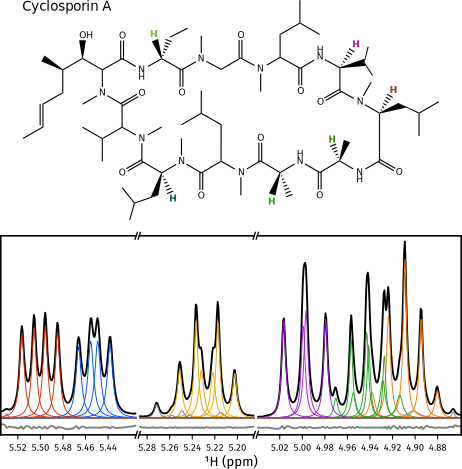
\includegraphics{/tmp/figure.pdf}
\end{center}

% blurb
\small
\begin{tcolorbox}[hbox]
\begin{varwidth}{\textwidth}
Estimation performed using \textsc{NMR-EsPy}.\\
Author: Simon Hulse\\
For more information:\\[5pt]
{\raisebox{-4pt}{\includegraphics[scale=0.029]{/home/simon/Documents/DPhil/projects/spectral_estimation/NMR-EsPy/nmrespy/images/book_icon.png}}}\hspace{1em}\href{https://foroozandehgroup.github.io/NMR-EsPy}{\texttt{https://foroozandehgroup.github.io/NMR-EsPy}}\\[5pt]
{\raisebox{-4pt}{\includegraphics[scale=0.12]{/home/simon/Documents/DPhil/projects/spectral_estimation/NMR-EsPy/nmrespy/images/github.png}}}\hspace{1em}\href{https://github.com/foroozandehgroup/NMR-EsPy}{\texttt{https://github.com/foroozandehgroup/NMR-EsPy}}\\[5pt]
{\raisebox{-3pt}{\includegraphics[scale=0.015]{/home/simon/Documents/DPhil/projects/spectral_estimation/NMR-EsPy/nmrespy/images/email_icon.png}}}\hspace{1em}\href{mailto:simon.hulse@chem.ox.ac.uk?subject=NMR-EsPy query}{\texttt{simon.hulse@chem.ox.ac.uk}}\\[5pt]
If used in a publication, please cite:\\
\textit{No references yet...}
\end{varwidth}
\end{tcolorbox}

\end{document}
